\section{Software design}
%TODO der mangler fyld tekst
\subsection{UI}

\begin{figure}[H]
	\centering
	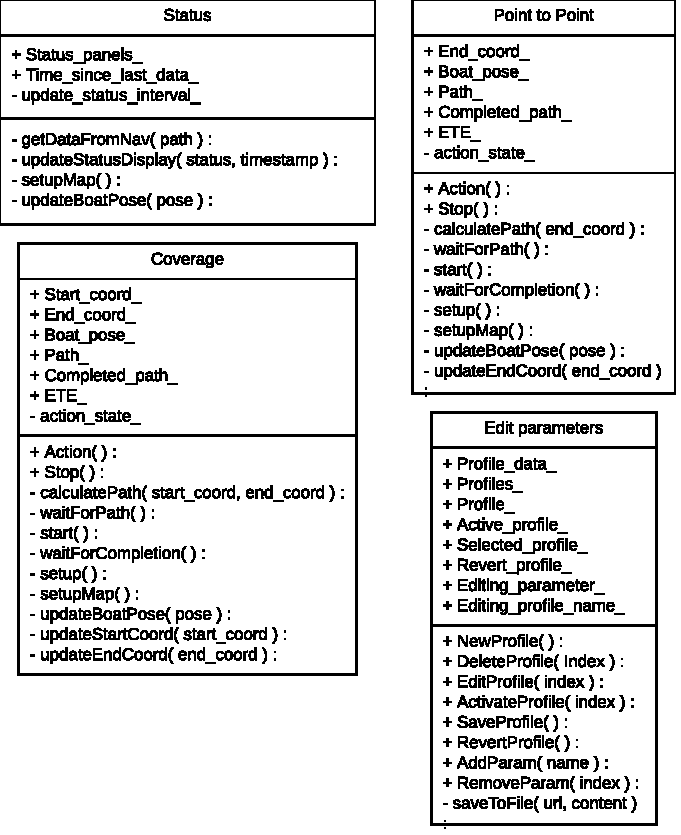
\includegraphics[width=1\linewidth]{Images/Design/User_Interface_overview}
	\caption{An overview of how the functions of the User Interface are structured}
	\label{fig:userinterfaceoverview}
\end{figure}


\subsubsection{Edit parameters}

\paragraph{Public methods:}
These public methods are called on click in the ui.
\begin{adjustwidth}{2.5em}{0pt}\begin{description}
	\item[NewProfile( )] creates a new profile object and appends it to the list of profiles, ie. the member \texttt{Profiles_}. This action then saves the \texttt{Profiles_} to a file.
	\item[DeleteProfile( index )] deletes the profile in the member \texttt{Profiles_} with the designated index. This action then saves the \texttt{Profiles_} to a file.
	\item[EditProfile( index )] displays the profile in the list \texttt{Profiles_} with the index, its profile name, parameters names and their values. \texttt{Revert_profile_} is set to contain the same values.
	\item[ActivateProfile( index )] sets the \texttt{Active_profile_} as the profile in \texttt{Profiles_} with the given index.
	\item[SaveProfile( )]  saves the \texttt{Profiles_} to a file, with the data in the data fields.
	\item[RevertProfile( )] sets \texttt{Profile_} to contain the same values as \texttt{Revert_profile_}.
	\item[AddParam( name )] adds a parameter to the parameter list in \texttt{Profile_}.
	\item[RemoveParam( index )] removes the parameter from the list of parameters in \texttt{Profile_} with the given index.
\end{description}\end{adjustwidth}


\paragraph{Private methods:}
\begin{adjustwidth}{2.5em}{0pt}\begin{description}
	\item[saveToFile( url, content )] sends a \texttt{POST} call to the server at the given url, with the content.
\end{description}\end{adjustwidth}

\paragraph{Public members:}
\begin{adjustwidth}{2.5em}{0pt}\begin{description}
	\item [Profile_data_] contains all the profiles in an encapsulating javascript object.
	\item [Profiles_] contains all the profiles, and resides in the \texttt{Profile_data_} object.
	\item [Profile_] is set to \texttt{Selected_profile_} when \texttt{EditProfile( )} is called.
	\item [Active_profile_] is the active profile.
	\item [Selected_profile_] is the selected profile in \texttt{Profiles_}.
	\item [Revert_profile_] holds the initial configuration of \texttt{Profile_}.
	\item [Editing_profile_] checks whether or not a profile is being edited.
	\item [Editing_profile_name_] checks whether or not a profile name is being edited.
\end{description}\end{adjustwidth}

\subsubsection{Status}

%TODO describe what a status object is in protocols

\paragraph{Private methods:}
\begin{adjustwidth}{2.5em}{0pt}\begin{description}
		\item [getDataFromNav( path )] sends a \texttt{GET} call to the server and gets the file at the path. It must include a status object and a time-stamp object to be valid.
		\item [updateStatusDisplay( status, timestamp )] should dynamically create the user interface elements that correspond to the different statuses in the status object. 
		\item [setupMap( )] sets up the map with appropriate settings.
		\item [updateBoatPose( pose )] updates the position and orientation of the boat on the map.
\end{description}\end{adjustwidth}

\paragraph{Public members:}
\begin{adjustwidth}{2.5em}{0pt}\begin{description}
		\item [Status_panels_] contains the \texttt{HTML} for the different statuses.
		\item [Time_since_last_data] contains how much time has passed since the last time-stamp, as well \texttt{CSS} class for the user interface, which colors the panel according to how much time has passed; blue recent, red dated, orange in between.
\end{description}\end{adjustwidth}


\paragraph{Private members:}
\begin{adjustwidth}{2.5em}{0pt}\begin{description}
		\item [update_status_interval_] is the delay between calls of the \texttt{getDataFromNav( )} function.
\end{description}\end{adjustwidth}


\subsubsection{Point to point}

\paragraph{Public methods:}
\begin{adjustwidth}{2.5em}{0pt}\begin{description}
		\item [Action( )] begins execution of the main task. \texttt{Action( )} first calculates the path, and then runs the path on the subsequent call if the \texttt{Path_} has been calculated. Likewise, the function will not calculate a new \texttt{Path_} before a previous \texttt{Path_} has been completed. 
		\item [Stop( )] stops execution by calling \texttt{saveToFile( )} and resets the state of the \texttt{Action( )} function by resetting \texttt{action_state_}.
\end{description}\end{adjustwidth}

\paragraph{Private methods:}
\begin{adjustwidth}{2.5em}{0pt}\begin{description}
		\item [calculatePath( end_coord )] writes the end_coord and function name to the \texttt{toNav.JSON} file. 
		\item [waitForPath( )] waits for a new \texttt{Path_} to be made available in the \texttt{fromNav.JSON} file, it checks this by way of time-stamps.
		\item [start( )] writes the function name to the \texttt{toNav.JSON} file, in order to tell the system to begin following the calculated \texttt{Path_}.
		\item [waitForCompletion( )] determines if the path has been completed, it does this by checking whether completion percentage is 100\%, coming from the \texttt{fromNav.JSON} file.
		\item [setup( )] sets up the some different variables, could thought of as the constructor.
		\item [setupMap( )] sets up the map with appropriate settings.
		\item [updateBoatPose( pose )] updates the position and orientation of the boat on the map.
		\item [updateEndCoord( end_coord )] updates the \texttt{End_coord_} with a new value.
\end{description}\end{adjustwidth}

%TODO describe polyline

\paragraph{Public members:}
\begin{adjustwidth}{2.5em}{0pt}\begin{description}
		\item [End_coord_] is the end point of the \texttt{Path_}.
		\item [Boat_pose_] is the position and orientation of the boat.
		\item [Path_] is a list of points which is interpreted as a polyline, and is the path that is intended to follow.
		\item[Completed_path_] is a list of points which is interpreted as a polyline, and is the path that the boat actually followed.
		\item[ETE_] contains the estimated time enroute, and the completion percentage, and a \texttt{CSS} class for dynamic styling. 
\end{description}\end{adjustwidth}


\paragraph{Private members:}
\begin{adjustwidth}{2.5em}{0pt}\begin{description}
		\item [action_state_] this is a counter that defines the state of the \texttt{Action( )} function.
\end{description}\end{adjustwidth}

\subsubsection{Coverage}

\paragraph{Public methods:}
\begin{adjustwidth}{2.5em}{0pt}\begin{description}
		\item [Action( )] begins execution of the main task. \texttt{Action( )} first calculates the path, and then runs the path on the subsequent call if the \texttt{Path_} has been calculated. Likewise, the function will not calculate a new \texttt{Path_} before a previous \texttt{Path_} has been completed. 
		\item [Stop( )] stops execution by calling \texttt{saveToFile( )} and resets the state of the \texttt{Action( )} function by resetting \texttt{action_state_}.
\end{description}\end{adjustwidth}

\paragraph{Private methods:}
\begin{adjustwidth}{2.5em}{0pt}\begin{description}
		\item [calculatePath( start_coord, end_coord )] writes the start_coord, end_coord, and function name to the \texttt{toNav.JSON} file. 
		\item [waitForPath( )] waits for a new \texttt{Path_} to be made available in the \texttt{fromNav.JSON} file, it checks this by way of time-stamps.
		\item [start( )] writes the function name to the \texttt{toNav.JSON} file, in order to tell the system to begin following the calculated \texttt{Path_}.
		\item [waitForCompletion( )] determines if the \texttt{Path_} has been completed, it does this by checking whether completion percentage is 100\%, coming from the \texttt{fromNav.JSON} file.
		\item [setup( )] sets up the some different variables, could thought of as the constructor.
		\item [setupMap( )] sets up the map with appropriate settings.
		\item [updateBoatPose( pose )] updates the position and orientation of the boat on the map.
		\item [updateStartCoord( start_coord )] updates the \texttt{Start_coord_} with a new value.
		\item [updateEndCoord( end_coord )] updates the \texttt{End_coord_ }with a new value.
\end{description}\end{adjustwidth}

\paragraph{Public members:}
\begin{adjustwidth}{2.5em}{0pt}\begin{description}
		\item [Start_coord_] is the start point of the coverage rectangle.
		\item [End_coord_] is the end point of the coverage rectangle.
		\item [Boat_pose_] is the position and orientation of the boat.
		\item [Path_] is a list of points which is interpreted as a polyline, and is the path that is intended to follow.
		\item[Completed_path_] is a list of points which is interpreted as a polyline, and is the path that the boat actually followed.
		\item[ETE_] contains the estimated time enroute, and the completion percentage, and a \texttt{CSS} class for dynamic styling. 
\end{description}\end{adjustwidth}


\paragraph{Private members:}
\begin{adjustwidth}{2.5em}{0pt}\begin{description}
		\item [action_state_] this is a counter that defines the state of the \texttt{Action( )} function.
\end{description}\end{adjustwidth}



\subsection{Controller}

\subsubsection{JSONReceiver}

\begin{figure}[H]
\centering
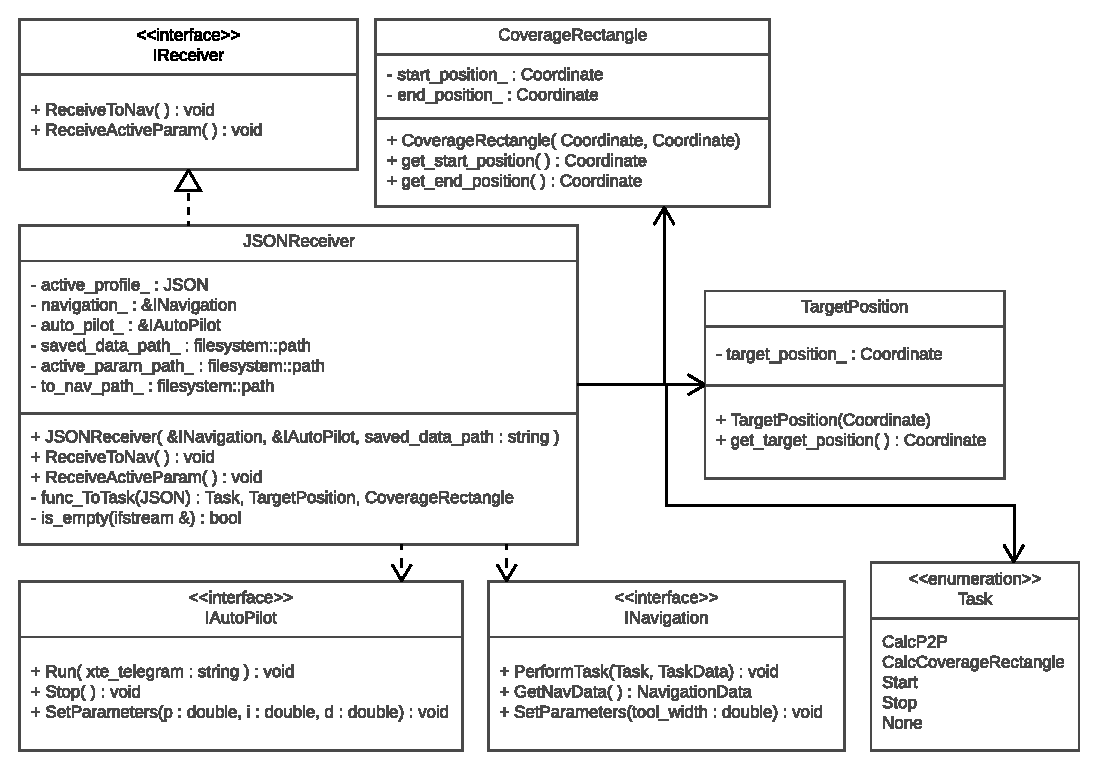
\includegraphics[width=1\linewidth]{Images/Design/Receiver_class_diagram}
\caption{Receiver class diagram}
\label{fig:Receiver}
\end{figure}

\paragraph{Public methods:}
\begin{adjustwidth}{2.5em}{0pt}\begin{description}
		\item [ReceiveToNav()] reads the toNav.json file
		\item [ReceiveActiveParam()] reads the activeParam.json file and sets the corresponding parameters in the Navigation and Autopilot
\end{description}\end{adjustwidth}

\paragraph{Private methods:}
\begin{adjustwidth}{2.5em}{0pt}\begin{description}
		\item [func_ToTask()] reads the task from the toNav.json file and calls the correct function overload of PerformTask in the Navigation
		\item [is_empty()] checks if a file is empty
\end{description}\end{adjustwidth}

\paragraph{Private members:}
\begin{adjustwidth}{2.5em}{0pt}\begin{description}
		\item [active_profile_] is a JSON object containing the current active parameter profile
		\item [navigation_] is a reference to a Navigation interface
		\item [auto_pilot_] is a reference to an Autopilot interface
		\item [saved_data_path_] is the filesystem path to the savedData folder in the website
		\item [active_param_path_] is the filesystem path to the active parameter JSON file
		\item [to_nav_path_] is the filesystem path to the toNav JSON file
\end{description}\end{adjustwidth}

\subsubsection{JSONTransmitter}

\begin{figure}[H]
\centering
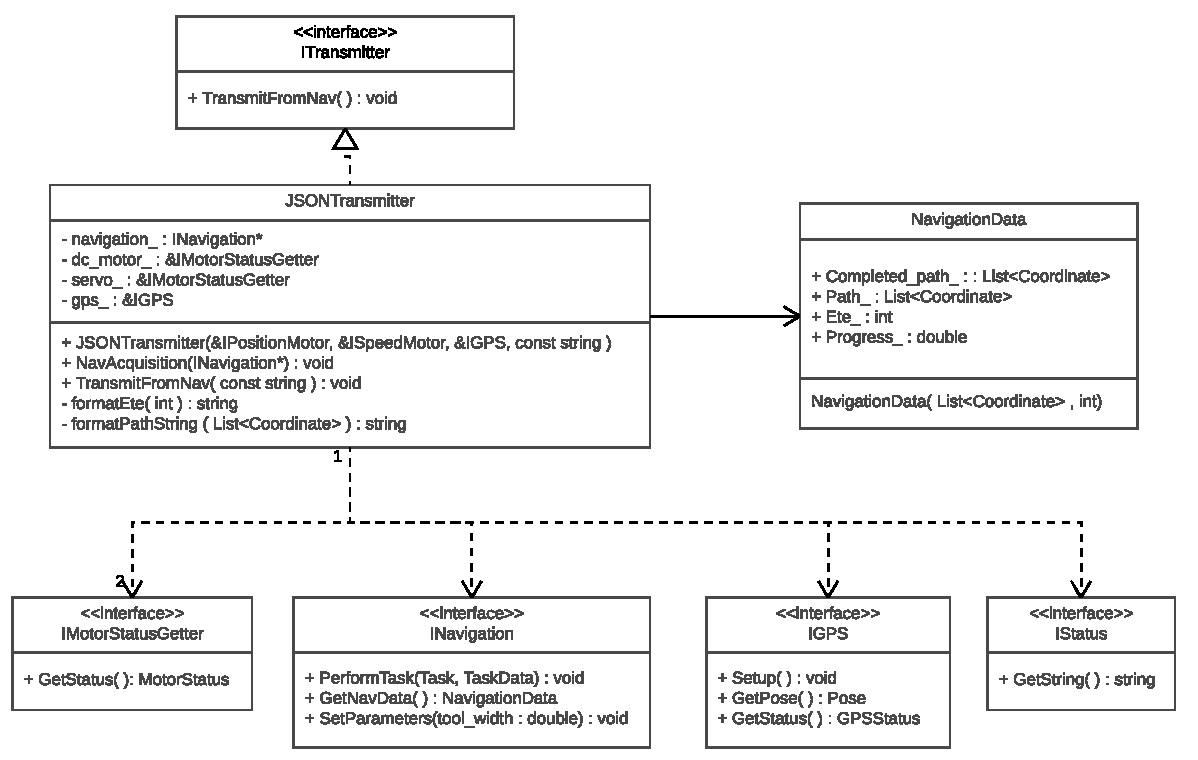
\includegraphics[width=1\linewidth]{Images/Design/Transmitter_class_diagram}
\caption{Transmitter class diagram}
\label{fig:Transmitter}
\end{figure}

\paragraph{Public methods:}
\begin{adjustwidth}{2.5em}{0pt}\begin{description}
		\item [NavAcquisition()] is a function to enable the Navigation and Transmitter unit to call each other. Since two classes can't have mutual references, the Transmitter is created first, the Navigation is then created with a reference to the Transmitter, and calls this function in its constructor. See the doxygen documents for more information on this method.
		\item [TransmitFromNav] is the point of the transmitter; transmitting the data the navigation unit has calculated. This function calls GetStatus in the motors and the GPS, as well as GetNavData on the Navigation unit to collect all the required data. It then packages it and writes to a JSON file. 
\end{description}\end{adjustwidth}

\paragraph{Private methods:}
\begin{adjustwidth}{2.5em}{0pt}\begin{description}
		\item [formatEte()] formats the estimated time enroute
		\item [formatPathString] formats the Path_ string received from the Navigation unit.
\end{description}\end{adjustwidth}

\paragraph{Private members:}
\begin{adjustwidth}{2.5em}{0pt}\begin{description}
		\item [navigation_] a pointer to a Navigation interface
		\item [dc_motor_] a reference to a MotorStatusGetter interface
		\item [servo_] a reference to a MotorStatusGetter interface
		\item [gps_] a reference to a GPS interface
\end{description}\end{adjustwidth}

\subsubsection{Navigation}

\begin{figure}[H]
\centering
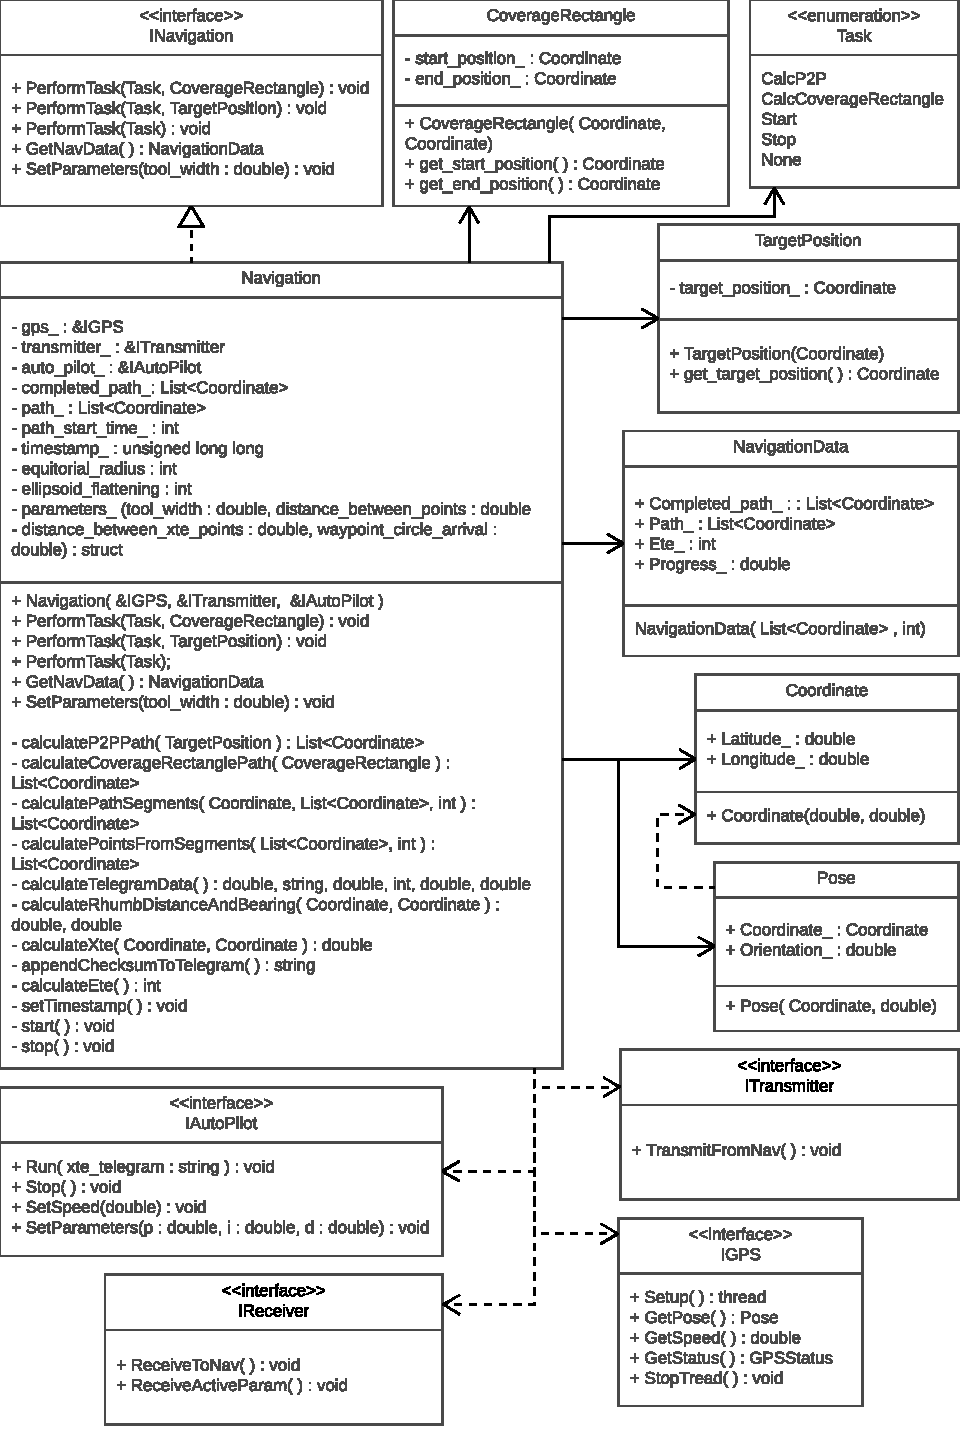
\includegraphics[width=1\linewidth]{Images/Design/Navigation_class_diagram}
\caption{Navigation class diagram}
\label{fig:Navigation}
\end{figure}

\paragraph{Public methods:}
\begin{adjustwidth}{2.5em}{0pt}\begin{description}
		\item [PerformTask()] is the first overload of the PerformTask function, and is called by the JSONReceiver if the current task is Start or Stop. In short, the function calls the start() or stop() functions, updates the timestamp_ and then calls the JSONTransmitter's TransmitFromNav function.
		\item [PerformTask()] is the second overload of the PerformTask function, and is called JSONReceiver if the current task is CalculateP2PPath. This function then calls calculateP2PPath(), and after a path has been calculated the timestamp_ will be set and the JSONTransmitter's TransmitFromNav function will be called.
		\item [PerformTask()] is the third overload of the PerformTask function, and is called JSONReceiver if the current task is CalculateCoverageRectanglePath. This function then calls calculateCoverageRectanglePath(), and after a path has been calculated the timestamp_ will be set and the JSONTransmitter's TransmitFromNav() function will be called.
		\item [GetNavData()] gets the Navigation data which is continually updated by the GPS.
		\item [SetParameters()] sets the parameters relevant for the Navigation unit, for example the tool_width of the survey equipment. All other relevant parameters could also be set here if wanted.
\end{description}\end{adjustwidth}

\paragraph{Private methods:}
\begin{adjustwidth}{2.5em}{0pt}\begin{description}
		\item [calculateP2PPath()] calculates a point to point path for the boat to traverse. 
		\item [calculateCoverageRectanglePath()] calculates a coverage rectangle path for the boat to traverse
		\item [calculatePathSegments()] calculates path segments for the current task, this is called by both calculateP2PPath() and calculateCoverageRectanglePath()
		\item [calculatePointsFromSegments()] calculates waypoints for the current task based on the previously calculated path segments. This is called by both calculateP2PPath() and calculateCoverageRectanglePath()
		\item [calculateTelegramData()] calculates data for the APB telegram which is sent to the Autopilot in the start() function
		\item [calculateRhumbDistanceAndBearing()] calculates the rhumb distance and absolute bearing between two coordinates
		\item [calculateXte()] calculates the cross track error for the boat, given the current position and path to follow
		\item [appendChecksumToTelegram()] calculates and appends a checksum to a telegram, then finishes the telegram
		\item [calculateEte()] calculates the estimated time enroute; the time the system expects it will take to reach the destination. This function uses the path_start_time_ and timestamp_ as well as the path_ and completed_path_ to give an estimate of this
		\item [setTimestamp()] sets the current millisecond timestamp in unix time
		\item [start()] calls calculateTelegramData(), then assembles the NMEA telegrams, calls appendChecksumToTelegram() for each telegram and then calls the Autopilot's Run() function with each telegram
		\item [stop()] calls Stop() in the Autopilot.
\end{description}\end{adjustwidth}

\paragraph{Private members:}
\begin{adjustwidth}{2.5em}{0pt}\begin{description}
		\item [gps_] a reference to a GPS interface
		\item [transmitter_] a reference to a Transmitter interface
		\item [auto_pilot_] a reference to an Autopilot interface
		\item [completed_path_] the completed part of the current Path_
		\item [path_] the current Path_ the boat has been asked to traverse by the user
		\item [path_start_time_] the start time of the current Path_. Used in calculateEte()
		\item [timestamp_] the timestamp of the last command completion
		\item [equitorial_radius_] the equitorial radius of the earht in the WGS84 standard
		\item [ellipsoid_flattening_] the ellipsoid flattening of the earht in the WGS84 standard
		\item [parameters_] the parameters of the system relevant for the Navigation unit
\end{description}\end{adjustwidth}

\subsubsection{Autopilot}

\begin{figure}[H]
\centering
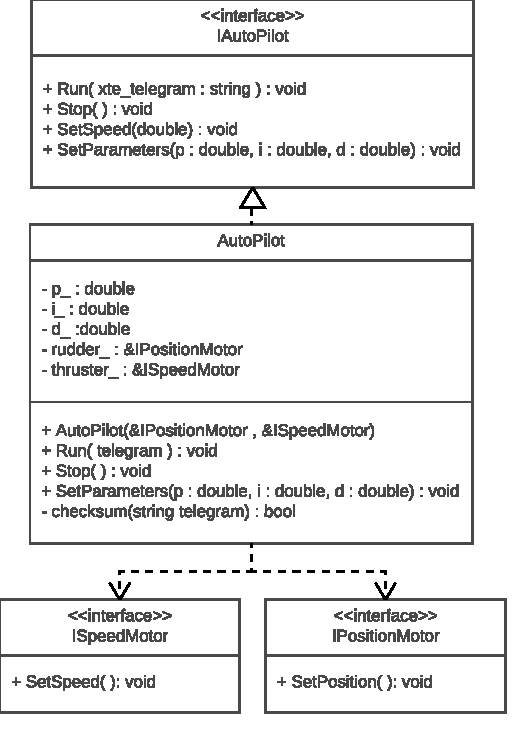
\includegraphics[width=1\linewidth]{Images/Design/Autopilot_class_diagram}
\caption{Autopilot class diagram}
\label{fig:Autopilot}
\end{figure}

\paragraph{Public methods:}
\begin{adjustwidth}{2.5em}{0pt}\begin{description}
		\item [Run()] gives the autopilot information about bearings, xte, which direction to turn, checkpoint number etc.
		\item [Stop()] tells the autopilot to stop the motors
		\item [SetParameters()] sets the PID parameters of the servo PID loop
\end{description}\end{adjustwidth}

\paragraph{Private methods:}
\begin{adjustwidth}{2.5em}{0pt}\begin{description}
		\item [checksum()] validates received NMEA messages by calculating and checking their checksum
\end{description}\end{adjustwidth}

\paragraph{Private members:}
\begin{adjustwidth}{2.5em}{0pt}\begin{description}
		\item [p_] is the product term of the position motor PID loop
		\item [i_] is the integral term of the position motor PID loop
		\item [d_] is the derivative term of the position motor PID loop
		\item [rudder_] is a reference to a position motor interface
		\item [thruster_] is a reference to a speed motor interface
\end{description}\end{adjustwidth}

\subsubsection{DCMotor}

%TODO fix pil
\begin{figure}[H]
\centering
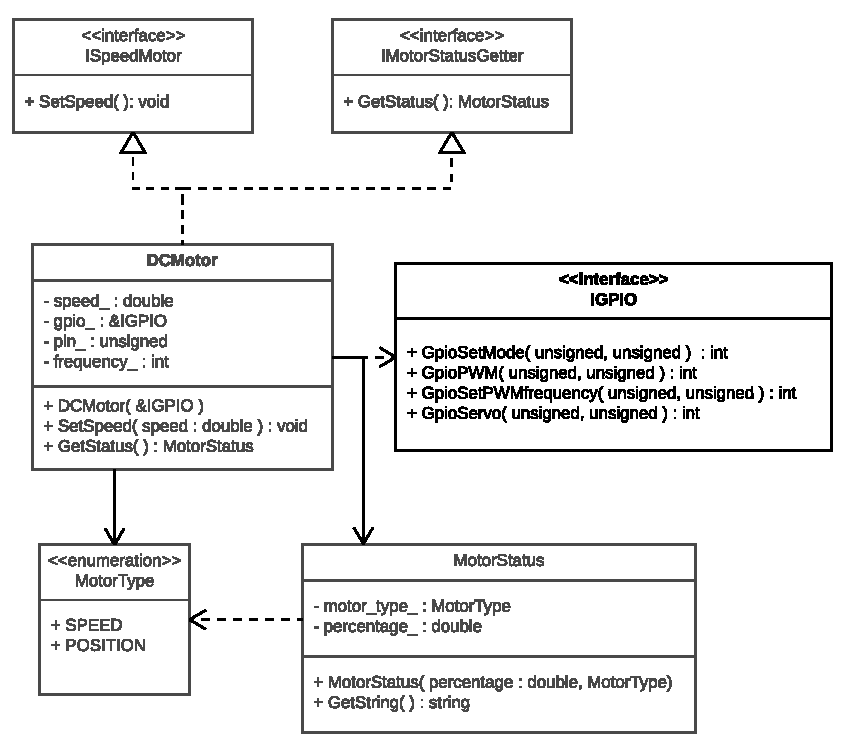
\includegraphics[width=1\linewidth]{Images/Design/DCMotor_class_diagram}
\caption{DCMotor class diagram}
\label{fig:dcmotor}
\end{figure}

\paragraph{Public methods:}
\begin{adjustwidth}{2.5em}{0pt}\begin{description}
		\item [SetSpeed()] sets the speed of the dc motor
		\item [GetStatus()] gets the status of the dc motor, a MotorStatus object
\end{description}\end{adjustwidth}

\paragraph{Private members:}
\begin{adjustwidth}{2.5em}{0pt}\begin{description}
		\item [speed_] the speed of the dc motor
		\item [gpio_] a reference to a GPIO object
		\item [pin_] the gpio the dc motor is controlled by
		\item [frequency_] the frequency of the dc motor
\end{description}\end{adjustwidth}

\subsubsection{Servo}

\begin{figure}[H]
\centering
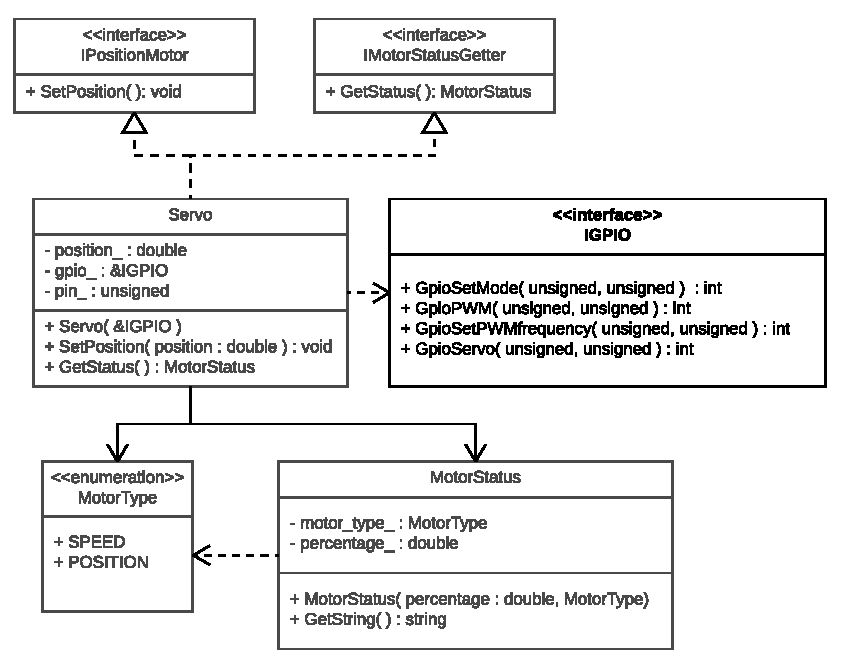
\includegraphics[width=1\linewidth]{Images/Design/Servo_class_diagram}
\caption{Servo class diagram}
\label{fig:servo}
\end{figure}

\paragraph{Public methods:}
\begin{adjustwidth}{2.5em}{0pt}\begin{description}
		\item [SetPosition()] sets the position of the servo
		\item [GetStatus()] gets the status of the servo, a MotorStatus object
\end{description}\end{adjustwidth}

\paragraph{Private members:}
\begin{adjustwidth}{2.5em}{0pt}\begin{description}
		\item [position_] the position of the servo
		\item [gpio_] a reference to a GPIO object
		\item [pin_] the gpio the servo is controlled by
\end{description}\end{adjustwidth}

\subsubsection{uBlox Neo 7-M}

\begin{figure}[H]
\centering
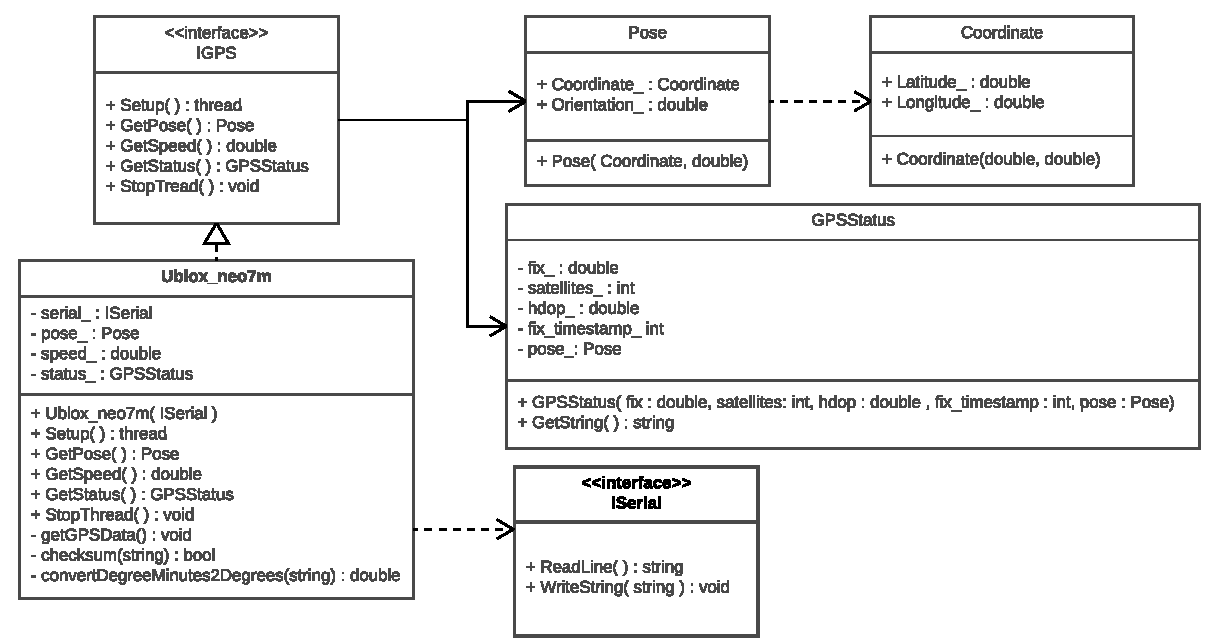
\includegraphics[width=1\linewidth]{Images/Design/ubloxNEO7M_class_diagram}
\caption{uBlox Neo 7-M class diagram}
\label{fig:ubloxneo7m}
\end{figure}

\paragraph{Public methods:}
\begin{adjustwidth}{2.5em}{0pt}\begin{description}
		\item [Setup()] sets up the GPS
		\item [GetPose()] gets the current pose
		\item [GetSpeed()] gets the current speed
		\item [GetStatus()] gets the current status
		\item [StopThread()] stops the asynchronous thread the GPS runs on
\end{description}\end{adjustwidth}

\paragraph{Private methods:}
\begin{adjustwidth}{2.5em}{0pt}\begin{description}
		\item [getGPSData()] gets the current GPS data
		\item [checksum()] validates received NMEA messages by calculating and checking their checksum
		\item [convertDegreesMinutes2Degrees()] converts between units
\end{description}\end{adjustwidth}

\paragraph{Private members:}
\begin{adjustwidth}{2.5em}{0pt}\begin{description}
		\item [serial_] is a serial interface
		\item [pose_] is the current pose
		\item [speed_] is the current speed
		\item [status_] is the current status of the GPS
\end{description}\end{adjustwidth}

\subsubsection{Helper classes}

\begin{figure}[H]
\centering
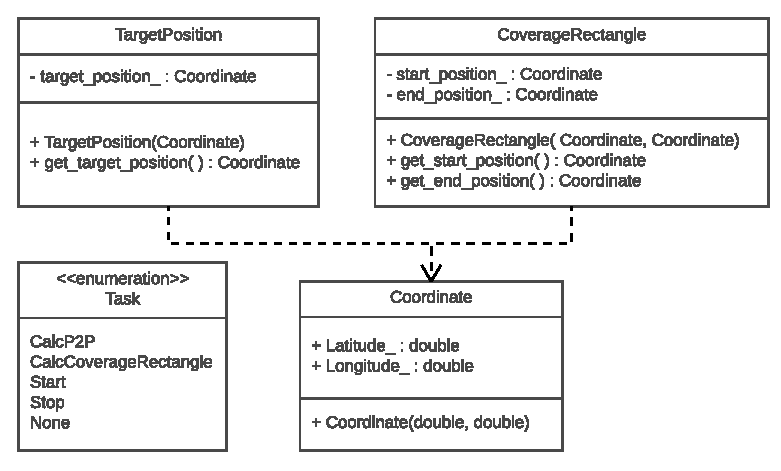
\includegraphics[width=1\linewidth]{Images/Design/Helpers_class_diagram}
\caption{Helpers class diagram}
\label{fig:helpers}
\end{figure}

\paragraph{Public methods:}
\begin{adjustwidth}{2.5em}{0pt}\begin{description}
		\item [get_target_position()] gets the target position
		\item [get_start_position()] gets the start position
		\item [get_end_position()] gets the end position
\end{description}\end{adjustwidth}

\paragraph{Public members:}
\begin{adjustwidth}{2.5em}{0pt}\begin{description}
		\item [Latitude_] is the latitude of a Coordinate
		\item [Longitude_] is the longitude of a Coordinate
\end{description}\end{adjustwidth}

\paragraph{Private members:}
\begin{adjustwidth}{2.5em}{0pt}\begin{description}
		\item [target_position_] is a coordinate with the target position
		\item [start_position_] is a coordinate with the starting position for a coverage rectangle
		\item [end_position_] is a coordinate with the end position for a coverage rectangle
\end{description}\end{adjustwidth}

\subsubsection{Status classes}

\begin{figure}[H]
\centering
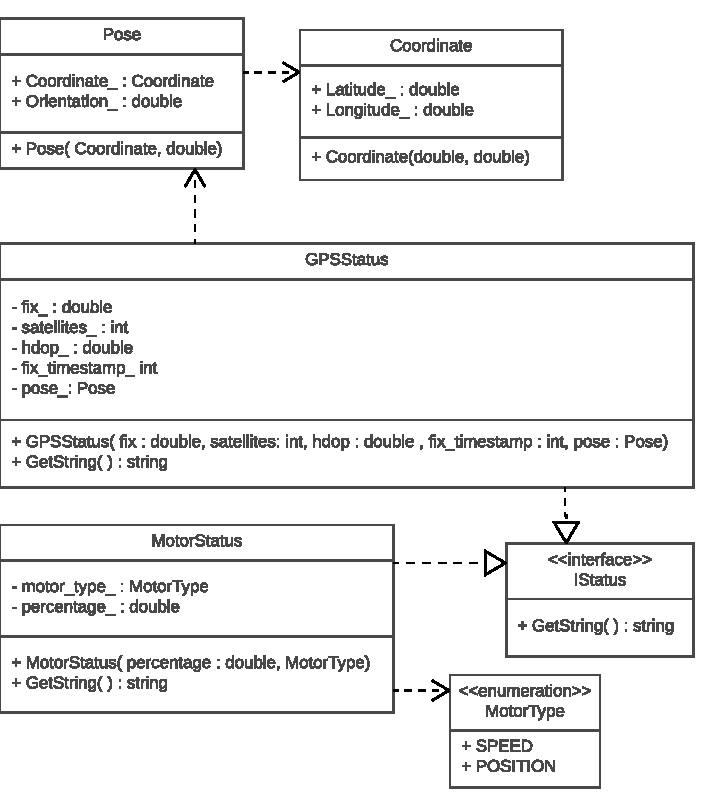
\includegraphics[width=1\linewidth]{Images/Design/Status_class_diagram}
\caption{Status class diagram}
\label{fig:status}
\end{figure}

\paragraph{Public methods:}
\begin{adjustwidth}{2.5em}{0pt}\begin{description}
		\item [GetString()] of the GPSStatus outputs a string with the GPS information, and is called by the JSONTransmitter
		\item [GetString()] of the MotorStatus outputs a string with the motor information, and is called by the JSONTransmitter
\end{description}\end{adjustwidth}

\paragraph{Public members:}
\begin{adjustwidth}{2.5em}{0pt}\begin{description}
		\item [Coordinate_] is the Coordinate of the current position of the boat 
		\item [Orientation_] is the orientation, or current absolute bearing of the boat
\end{description}\end{adjustwidth}

\paragraph{Private members:}
\begin{adjustwidth}{2.5em}{0pt}\begin{description}
		\item [fix_] describes the fix level of the GPS
		\item [satellites_] is how many satellites the GPS is currently receiving from
		\item [hdop_] is the horizontal dilution of precision
		\item [fix_timestamp_] is the timestamp of the current fix 
		\item [pose_] is the pose of the boat
		\item [motor_type_] is the type of motor for a MotorStatus
		\item [percentage_] is the percentage (0-100) for a given motor
\end{description}\end{adjustwidth}